\documentclass[12pt, a4paper]{article}
\usepackage{lmodern}
\usepackage[utf8]{inputenc}
% \usepackage{fontspec}
\usepackage{amssymb,amsmath}
\usepackage[T1]{fontenc}
\usepackage[scale=0.8]{geometry} 
\usepackage[french]{babel}% pour un document en français.
\usepackage{minted}
\usepackage{graphicx}
\usepackage[colorlinks=true, linkcolor=blue]{hyperref}
\date{}
\title{Rapport de TP de Technologie Web Serveur}
\author{Loïc \textsc{Castillo} Loris \textsc{Croce}}

\begin{document}

\maketitle

\paragraph{Base de donnée} Il est possible d'initialiser une base de donnée de test via le fichier \verb|requetes.sql|

\section{Conception}

\begin{figure}[!h]
   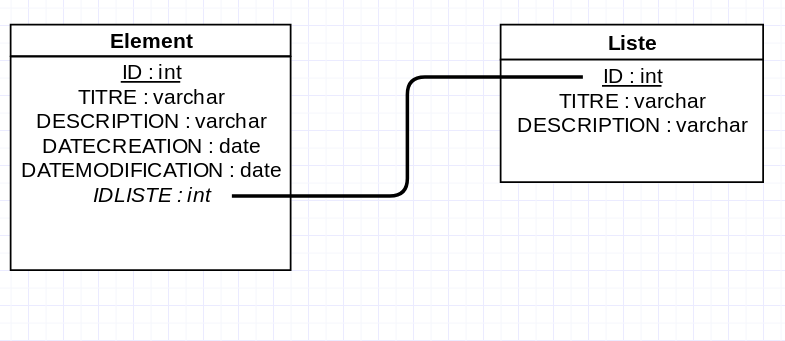
\includegraphics[width=15cm]{donnees.png}
   \caption{Modèle de données}
\end{figure}

\paragraph{Ressources} On interagira avec des listes et des éléments qui pourront être affichés (un élément affiché dans une liste), ajoutés, supprimés et modifiés.

\paragraph{Espaces de noms}
\begin{itemize}
\item  Pour l'affichage seules les listes auront une URL de la forme : \texttt{/liste/\emph{nomDeLaListe}}.
\item Pour supprimer une ressource de type :
	\begin{itemize} 
	\item liste, l'URL sera de la forme : \texttt{/supprimerListe/\emph{nomDeLaListe}}
	\item élément : \texttt{/supprimerElement/\emph{nomDeLaListe}/\emph{nomDeL'Element}}
	\end{itemize}
\item Pour créer une ressource de type :
	\begin{itemize} 
	\item liste, l'URL sera de la forme : \texttt{/creerListe}
	\item élément : \texttt{/creerElement}
	\end{itemize}
\item Pour modifier une ressource de type :
	\begin{itemize} 
	\item liste, l'URL sera de la forme : \texttt{/modifierListe}
	\item élément : \texttt{/\emph{nomDeLaListe}/modifierElement}
	\end{itemize}

\end{itemize}

\section{Modèle et accès au données}

Nous avons donc deux classes métiers pour le modèle : \verb|Element| et \verb|Liste| définissant les deux objets manipulés.\\ 

Étant donné que le nombre d'appels à la base de données ne sera pas très élevé, nous avons décidé que notre DAO serait une classe statique. Les informations pour se connecter à la base de données sont stockées dans les variables de la classe. Chaque fonction retourne des objets métiers et est utilisée pour une tâche précise (ex: récupérer toutes les listes, les éléments, un élément particulier, les éléments en fonction de leur liste\dots). Chaque appel de fonction doit recréer une connexion à la base de données.

\section{Représentations}

Via FreeMarker, nous avons créé 3 templates :
\begin{itemize}
	\item \verb|complet.ftl|, qui affiche tous les éléments de toutes les listes.
	\item \verb|listeDetail.ftl|, qui affiche une liste donnée et tous ses éléments. Elle permet de supprimer ou de modifier des éléments.
	\item \verb|listes.ftl|, qui fait office de page ``d'accueil'' en affichat un tableau des listes. Elle permet également de d'ajouter, modifier ou supprimer des listes, ajouter des éléments.
\end{itemize}

\section{Interactions}

Pour la gestion des interactions par le contrôleur avec Spark nous n'avons utilisé que deux méthodes HTTP : GET et POST. En effet, la gestion de méthodes telles que DELETE ou PATCH ne s'est pas révelée assez pertinente en raison de leur plus complexe mise en place car les formulaires HTML ne gèrent pas les autres types de requêtes. On a donc un ensemble de \emph{routes} de types \verb|get| pour récupérer du contenu ou supprimer des élements (on affiche la liste en enlevant l'élement voulu). Ainsi qu'un ensemble de \emph{routes} \verb|post| pour créer ou modifier du contenu.

\section{Ajout de fonctionnalités}

\paragraph{Statut optionnel} Il suffit d'ajouter une table \verb|Etat| dans la base de données, contenant un id et un varchar, qui contiendrait 3 tuples, dont la valeur des varchar serait : soit \emph{à faire}, \emph{fait} ou \emph{supprimé}.

\paragraph{Sous-listes}
Dans la BDD, la table \verb|Liste|, aurait une colonne \verb|Upper|, qui contiendrait l'ID d'une autre liste, ou serait NULL.
En Java, cela se matérialiserait par l'ajout d'une List de Liste dans la classe Liste. Celle-ci serait vide si l'attribut est NULL dans la BDD.

\paragraph{Élément appartenant à plusieurs listes}
Dans la BDD, il faudrait créer une table de liaison, qui lirait deux listes. On pourrait l'appeler \verb|ListJunction|, et serait composer de deux id de Liste. L'ajout de ces deux id donneraient la clé primaire de l'élément.

\paragraph{Étiquette} L'ajout de tags sera plus complexe que le reste. Cela nécessitera deux tables dans la Base de Données. Une première pour gérer les tags, avec un id et un varchar, contenant le texte du tag correspondant. Et une seconde table pour faire la liaison entre un élément et un tag. Celle-ci contiendra deux clés étrangères : Celle du tag et celle d'un élément. La concaténation de ces deux attributs donnera la clé primaire. En Java, il suffira simplement d'ajouter une liste de String à chaque élément. Celle-ci sera vide pour les elements n'ayant pas encore été taggé.


\end{document}